\documentclass[12pt,letterpaper]{article}
\usepackage{inverba}
\newcommand{\userName}{Cullyn Newman}
\newcommand{\class}{BI 336} 
\newcommand{\institution}{Portland State University} 
\newcommand{\thetitle}{\hypertarget{home}{Cellular Biology}}
\rfoot{\hyperlink{home}{10 --- \thepage}}

\begin{document}
%%%%%%%%%%%%%%%%%%%%%%%%%%%%%%%%%%%%%%%%%%%%%%%%%%%%%%%%%%%%%%%%%%%%%%%%%%%%%%%%%%%%%%%%%
%                               %   %   %   %   %   %   %                               %
%                           %   %   %   %   %   %   %   %   %                           %
%                       %   %                               %   %                       %
%   %   %   %   %   %   %   %   O   U   T   L   I   N   E   %   %   %   %   %   %   %   %
%                       %   %                               %   %                       %
%                           %   %   %   %   %   %   %   %   %                           %
%                               %   %   %   %   %   %   %                               %
%%%%%%%%%%%%%%%%%%%%%%%%%%%%%%%%%%%%%%%%%%%%%%%%%%%%%%%%%%%%%%%%%%%%%%%%%%%%%%%%%%%%%%%%%

%\begingroup

\begin{chapbox}{Cellular Biology}{ 
\begin{enumerate}[font=\bfseries, wide]
    \setcounter{enumi}{9}
    \item \hyperlink{10}{\textbf{Membrane Structure}}
    \begin{itemize}
        \item \hyperlink{10.1}{The Lipid Bilayer}
        \item \hyperlink{10.2}{Membrane Proteins}
    \end{itemize}
    \item \hyperlink{11}{\textbf{Transport Across Membrane}}
    \begin{itemize}
        \item
    \end{itemize}
    \item \hyperlink{12}{\textbf{Intracellular Transport}}
    \begin{itemize}
        \item 
    \end{itemize}
    \item \hyperlink{13}{\textbf{Vesicular Trafficking, Secretion, \& Endocytosis}}
    \begin{itemize}
        \item
    \end{itemize}
    \item \hyperlink{14}{\textbf{Energy Conversion: Mitochondria and Chloroplasts}}
    \begin{itemize}
        \item 
    \end{itemize}
    \item \hyperlink{15}{\textbf{Cellular Communication}}
    \begin{itemize}
        \item 
    \end{itemize}
    \item \hyperlink{16}{\textbf{The Cytoskeleton}}
    \begin{itemize}
        \item 
    \end{itemize}
    \item \hyperlink{17}{\textbf{The Cell Cycle}}
    \begin{itemize}
        \item 
    \end{itemize}
    \item \hyperlink{18}{\textbf{Apoptosis}}
    \begin{itemize}
        \item 
    \end{itemize}
    \item \hyperlink{19}{\textbf{Cell Interactions}}
    \begin{itemize}
        \item 
    \end{itemize}
    \item \hyperlink{20}{\textbf{Cancer}}
    \begin{itemize}
        \item 
    \end{itemize}    
    \item[22.] \hyperlink{22}{\textbf{Stem Cells and Tissue Renewal}}
    \begin{itemize}
        \item 
    \end{itemize}
    \item[24.] \hyperlink{24}{\textbf{The Innate and Adaptive Immune System}}
    \begin{itemize}
        \item 
    \end{itemize}
\end{enumerate}
}\end{chapbox}
\clearpage
%\endgroup

%%%%%%%%%%%%%%%%%%%%%%%%%%%%%%%%%%%%%%%%%%%%%%%%%%%%%%%%%%%%%%%%%%%%%%%%%%%%%%%%%%%%%%%%%
%                               %   %   %   %   %   %   %                               %
%                           %   %   %   %   %   %   %   %   %                           %
%                       %   %                               %   %                       %
%   %   %   %   %   %   %   %       N   O   T   E   S       %   %   %   %   %   %   %   %
%                       %   %                               %   %                       %
%                           %   %   %   %   %   %   %   %   %                           %
%                               %   %   %   %   %   %   %                               %
%%%%%%%%%%%%%%%%%%%%%%%%%%%%%%%%%%%%%%%%%%%%%%%%%%%%%%%%%%%%%%%%%%%%%%%%%%%%%%%%%%%%%%%%%


%%%%%%%%%%%%%%%%%%%%%%%%%%%%%%%%%%%%%%%%%%%%%%%%%%%%%%%%%%%%%%%%%%%%%%%%%%%%%%%%%%%%%%%%%%
%  vvvvvvvvvvvvvvvvvvvvvvvvvvvvvvvvv   Section 10.1   vvvvvvvvvvvvvvvvvvvvvvvvvvvvvvvvv  %
%\begingroup


\renewcommand{\thetitle}{\hypertarget{10}{The Genetic Code of Genes
and Genomes}}
\rfoot{\hyperlink{10}{10 --- \thepage}}
\hypertarget{10}{} 

%%%%%%%%%%%%%%%%%%%%%%%%%%%%%%%%%%%%%%%%%%%%%%%%%%%%%%%%%%%%%%%%%%%%%%%%%%%%%%%%%%%%%%%%%

\begin{chapbox}{\hyperlink{home}{Chapter 10: The Cell Membrane}}
    \begin{enumerate}
        \item \hyperlink{10.1}{The Lipid Bilayer}
        \item \hyperlink{10.2}{Membrane Proteins}
    \end{enumerate}
\end{chapbox}

\hypertarget{10.1}{}
\begin{secbox}{\hyperlink{10}{The Lipid Bilayer}}{
    \subsection*{Phosphoglycerides, Sphingolipids, and Sterols Are the Major
    Lipids in Cell Membranes}
    \begin{itemize}
        \item \textbf{Plasma membrane}: the part of the cell that separates the exterior and the interior of a cell with a semipermeable lipid bilayer. The plasma membrane regulates import and export of materials for the cell and includes various proteins that interact with other cells. 
        \item \textbf{Lipid bilayer}: the resulting structure of the spontaneous alignment of mostly amphiphilic phospholipids. 
        \item \textbf{Amphiphilic}: a chemical compound possessing a polar \textbf{hydrophilic} component and a \textbf{hydrophobic}, or lipophilic (fat loving), non polar end.
        \item \textbf{Phospholipids}: the most abundant membrane lipid containing a polar head consisting of a phosphate group and two hydrophobic fatty acid tails made of hydrocarbons.
        \item \textbf{Phosphoglycerides}: the main compounds that make up the phospholipids in animal cells, consisting of have a three-carbon glycerol backbone. Different combinations of head groups and tails can yield different phosphoglycerides. The most notable are: phosphatidylethanolamine, phosphatidylserine, and phosphatidylcholine.
        \item \textit{Sphingolipids}: similar to phosphoglycerides, but made up of sphingosine rather than glycerol.
        \item \textbf{Cholesterol}: a \textit{sterol} containing a rigid ring structure and attached to a single polar hydroxyl group. Cholesterol sits in the middle of the bilayer and helps provide structure by reducing tail mobility. 
    \end{itemize}

    \subsection*{The Lipid Bilayer Is a Two-dimensional Fluid}
    \begin{itemize}   
        \item \textbf{Liposomes}: a spherical with at least one lipid bilayer, most often made up of phospholipids, especially phosphatidylcholine.
        \item \textit{Phospholipid translocators}, or flippases, move phospholipids from the exoplasmic face (outside), to the cytosolic face (inside) of a lipid bilayer. Floppases move phospholipids in the inverse direction. 
        \item Fluidity depends on both composition and temperature. 
        \item \textit{Cis}-double bonds form kinks in the hydrocarbon tails, which make it harder to the tails to fit uniformly and constant movement within the bilayer.
        \item The addition of cholesterol decrease fluidity, but at the same time, high concentrations found in most eukaryotic plasma membranes also prevents the hydrocarbon chains from coming together and crystallizing.\par
        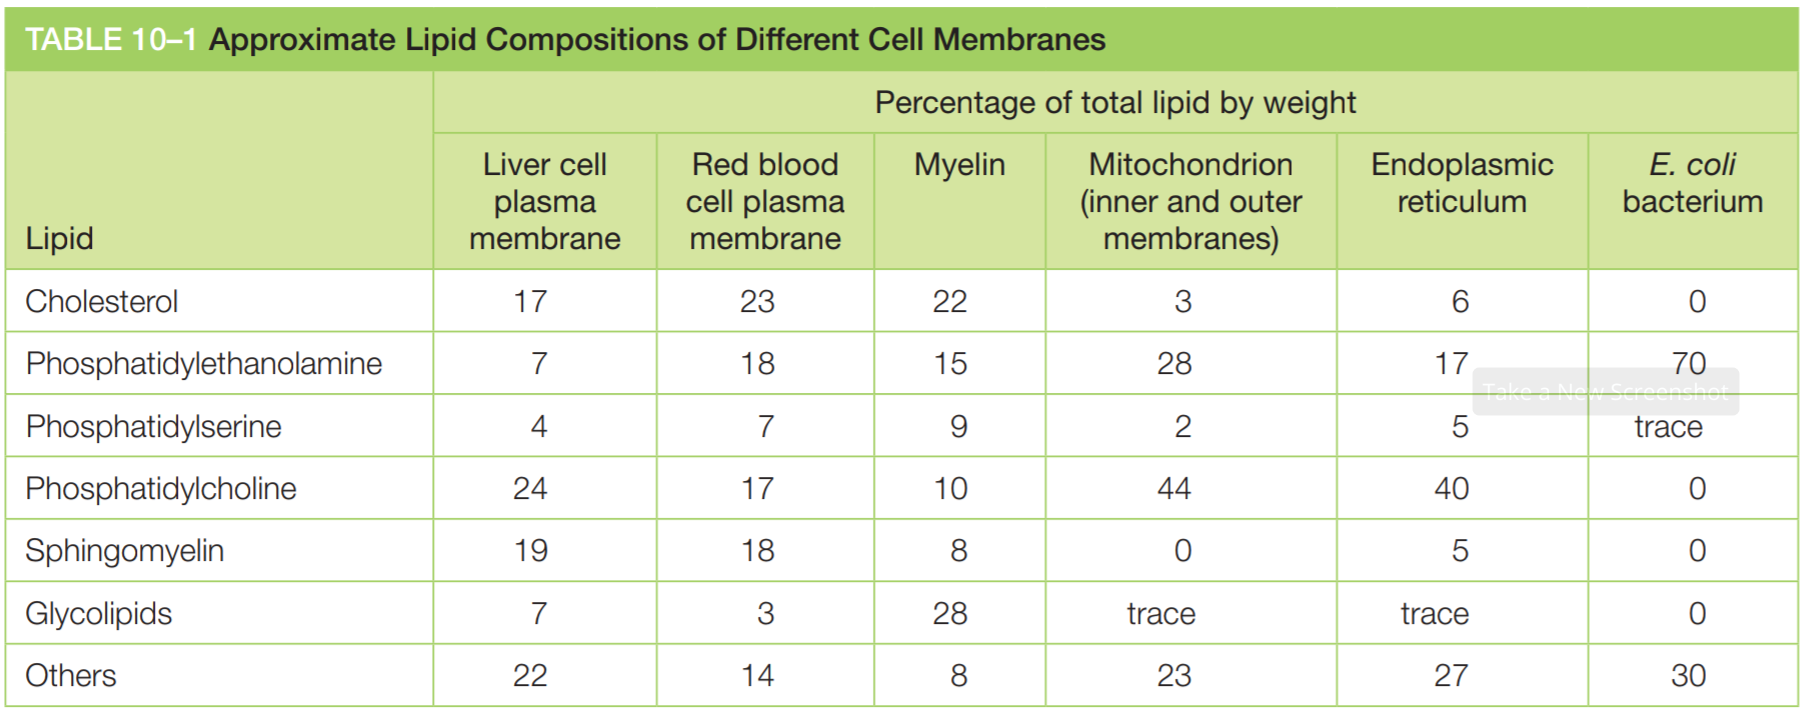
\includegraphics[width=\linewidth]{images/table_10_1.png}
    \end{itemize}

    \subsection*{Despite Their Fluidity, Lipid Bilayers Can Form Domains of Different Compositions}
    \begin{itemize}
        \item \textbf{Lipid raft}: specialized domains, or regions, that are enriched with particular lipids and cholesterol that allow for specialized associations with different cellular proteins. 
        \item Lipid rafts are dynamic structures, often coming together or splitting apart.\
        \item Lipid rafts influence membrane fluidity and membrane protein trafficking,
        \item Although more common in the cell membrane, lipid rafts have also been reported in other parts of the cell, such as the Golgi apparatus and lysosomes.
    \end{itemize}

    \subsection*{Lipid Droplets Are Surrounded by a Phospholipid Monolayer}
    \begin{itemize}
        \item \textbf{Lipid droplets}: lipid-rich cellular organelles that regulate the storage and hydrolysis of neutral lipids and are found largely in the adipose (fat) tissue. 
        \item Lipid droplets also serve as a reservoir for cholesterol and acyl-glycerols for membrane formation and maintenance.
        \item Generally, lipid droplets form rapidly in high concentration of fatty acids and generally form from discrete regions of the endoplasmic reticulum membrane where many enzymes of lipid metabolism are concentrated.
    \end{itemize}

    \subsection*{The Asymmetry of the Lipid Bilayer Is Functionally Important}
    \begin{itemize}
        \item The lipid compositions of the two monolayers of the lipid bilayer in many membranes are strikingly different.
        \item Lipid asymmetry is functionally important, especially in converting extracellular signals into intracellular ones, as many cytosolic proteins bind to specific lipid head groups found in the cytosolic monolayer of the lipid bilayer. 
        \item Animals exploit the phospholipid asymmetry of their plasma membranes to
        distinguish between live and dead cells. 
    \end{itemize}
    
    \subsection*{Glycolipids Are Found on the Surface of All Eukaryotic Plasma Membranes}
    \begin{itemize}
        \item \textbf{Glycolipids}: lipids with a carbohydrate attached by a glycosidic (covalent) bond.
        \item Glycolipids maintain the stability of the cell membrane and to facilitate cellular recognition, and are found on the surface of probably all eukaryotic cell membranes, where they extend from the phospholipid bilayer into the extracellular environment. 
        \item Glycolipids generally constitute about 5\% of the lipid molecules in the outer monolayer. 
        \item \textbf{Gangliosides}: a glycolipid that contain oligosaccharides (a polymer contain typically three to ten monosaccharides) with one or more sialic acid (an acidic sugar with a nine-carbon backbone), which produce a net negative charge.
        \item  Gangliosides are found predominantly in the nervous system where they constitute 6\% of all phospholipids.
    \end{itemize}

    \begin{probbox}{The Lipid Bilayer: Summary}
        Biological membranes consist of a continuous double layer of lipid molecules in which membrane proteins are embedded. This lipid bilayer is fluid, with individual lipid molecules able to diffuse rapidly within their own monolayer. The membrane lipid molecules are amphiphilic. When placed in water, they assemble spontaneously into bilayers, which form sealed compartments. Although cell membranes can contain hundreds of different lipid species, the plasma membrane in animal cells contains three major classes—phospholipids, cholesterol, and glycolipids. Because of their different backbone structure, phospholipids fall into two subclasses—phosphoglycerides and sphingolipids. The lipid compositions of the inner and outer monolayers are different, reflecting the different functions of the two faces of a cell membrane. Different mixtures of lipids are found in the membranes of cells of different types, as well as in the various membranes of a single eukaryotic cell. Inositol phospholipids are a minor class of phospholipids, which in the cytosolic leaflet of the plasma membrane lipid bilayer play an important part in cell signaling: in response to extracellular signals, specific lipid kinases phosphorylate the head groups of these lipids to form docking sites for cytosolic signaling proteins, whereas specific phospholipases cleave certain inositol phospholipids to generate small intracellular signaling molecules.
    \end{probbox}
}\end{secbox}
%  ^^^^^^^^^^^^^^^^^^^^^^^^^^^^^^^^^   Section 10.1   ^^^^^^^^^^^^^^^^^^^^^^^^^^^^^^^^  %  
%%%%%%%%%%%%%%%%%%%%%%%%%%%%%%%%%%%%%%%%%%%%%%%%%%%%%%%%%%%%%%%%%%%%%%%%%%%%%%%%%%%%%%%%%%
%  vvvvvvvvvvvvvvvvvvvvvvvvvvvvvvvvvv  Section 10.2   vvvvvvvvvvvvvvvvvvvvvvvvvvvvvvvv  % 
\hypertarget{10.2}{}
\begin{secbox}{\hyperlink{10}{Membrane Proteins}}{
    \subsection*{Membrane Proteins Can Be Associated with the Lipid Bilayer in Various Ways}
    \begin{itemize}
        \item \textbf{Membrane proteins}: amphiphilic proteins that are part of, or interact with, biological membranes. 
        \item Membrane proteins fall into several broad categories depending on their location, and classified generally as either integral or peripheral.
        \item Integral membrane proteins are a permanent part of a cell membrane and can either penetrate the membrane (transmembrane) or associate with just a single side of a membrane (integral monotopic).
        \item \textbf{Transmembrane protein}: a type of integral membrane protein that spans the entirety of the cell membrane.
        \item Transmembrane proteins are usually highly hydrophobic and aggregate and precipitate in water.
        \item Depending on the number of transmembrane segments, transmembrane proteins can be classified as single-span (or bitopic) or multi-span (polytopic).
        \item \textbf{Glycosylphosphatidylinositol (GPI) anchor}: a phosphoglyceride that can be attached to the C-terminus of a protein.
        \item The two fatty acids within the hydrophobic phosphatidyl-inositol group GPI anchor the protein to the cell membrane; leaving the protein bound to the noncytosolic surface of the ER membrane solely by this anchor.
        \item \textbf{Membrane-associated proteins}: proteins that do not extend into the hydrophobic interior of the lipid bilayer at all; they are instead bound to either face of the membrane by noncovalent interactions with other membrane proteins.\par
        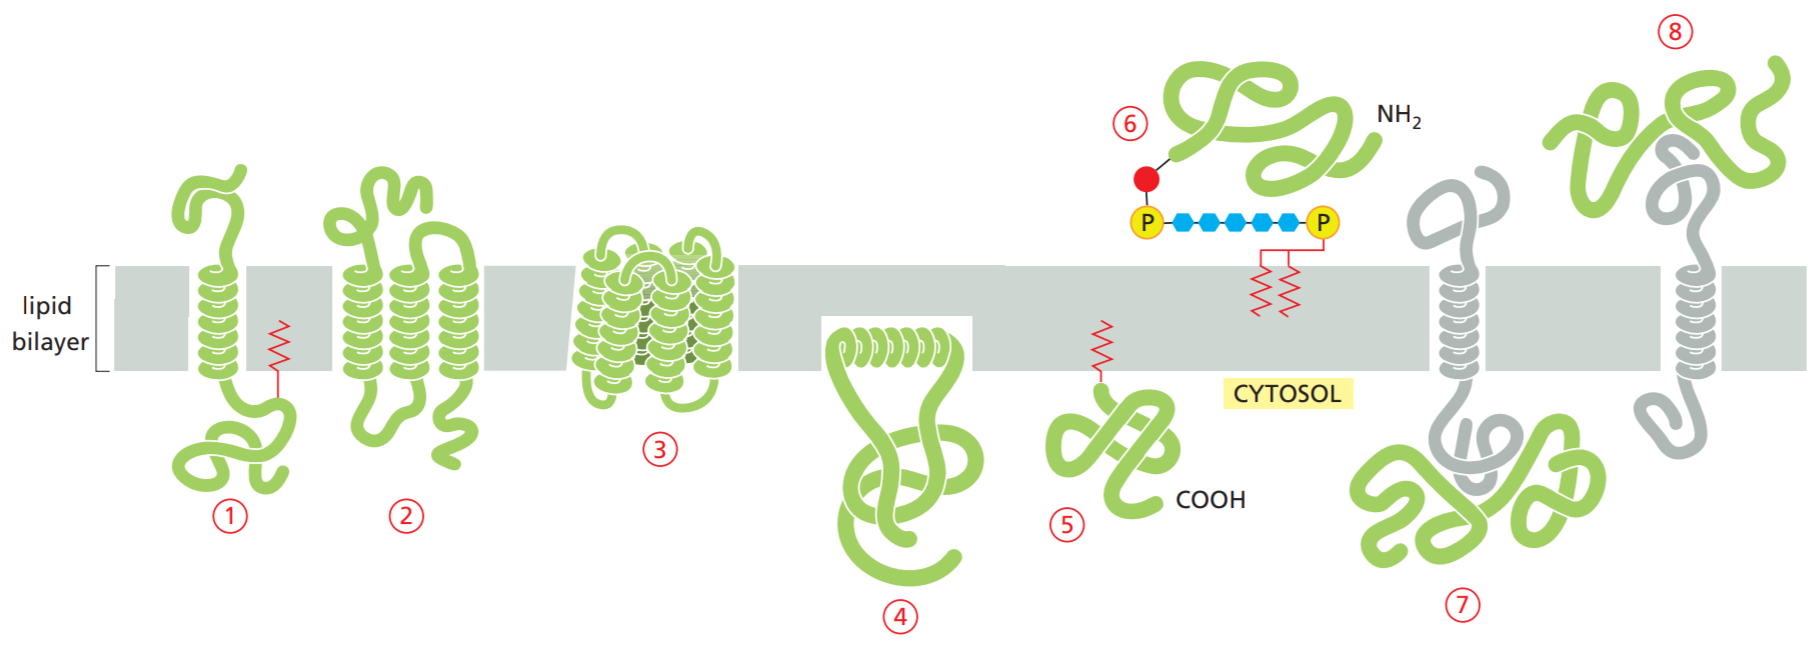
\includegraphics[width=\linewidth]{images/figure_10_17.png}
        \item \textcolor{red}{(1)} a single \(\alpha\) helix
        \item \textcolor{red}{(2)} as multiple \(\alpha\) helices
        \item \textcolor{red}{(3)} as a rolled-up \(\beta\) sheet (a \(\beta\) barrel). 
        \item \textcolor{red}{(4)} Some of these are anchored to the cytosolic surface by an amphiphilic \(\alpha\) helix that partitions into the cytosolic monolayer of the lipid bilayer through the hydrophobic face of the helix. 
        \item \textcolor{red}{(5)} Others are attached to the bilayer solely by a covalently bound lipid chain—either a fatty acid chain or a phenyl group in the cytosolic monolayer.
        \item \textcolor{red}{(6)} via an oligosaccharide linker, to phosphatidylinositol in the noncytosolic monolayer—called a GPI anchor. 
        \item \textcolor{red}{(7, 8)} membrane-associated proteins are attached to the membrane only by noncovalent interactions with other membrane proteins.
    \end{itemize}
    
    \subsection*{Lipid Anchors Control the Membrane Localization of Some Signaling Proteins}
    \begin{itemize}
        \item \textit{Prenyl groups}: usually to facilitate attachment to cell membranes, similar to lipid anchors like the GPI anchor. Also can be done by a fatty acid chain.
        \item Prenyl groups have been shown to be important for protein–protein binding through specialized prenyl-binding domains.
    \end{itemize}
    
    \subsection*{In Most Transmembrane Proteins, the Polypeptide Chain Crosses the Lipid Bilayer in an \(\bm{\alpha}\)-Helical Conformation}
    \begin{itemize}
        \item \textbf{Single pass transmembrane proteins} \textcolor{red}{(1)}: also known as bitopic proteins, which are transmembrane proteins that span the lipid bilayer only one time. 
        \item Bitopic proteins may constitute up to 50\% of all transmembrane proteins, depending on the organism, and contribute significantly to the network of interactions between different proteins in cells, including interactions via transmembrane helices.
        \item \textbf{Multi-pass transmembrane proteins} \textcolor{red}{(2)}: also known as polytopic proteins, where the polypeptide chain crosses membrane multiple times. 
    \end{itemize}

    \subsection*{Some \bfg{\beta} Barrels Form Large Channels}
    \begin{itemize}
        \item The number of \(\beta\)-strands in a \(\beta\)-barrel varies widely, from as few as 8 strands to as many as 22
        \item \(\beta\)-barrel proteins are abundant in the outer membranes of bacteria, mitochondria, and chloroplasts.
        \item \textbf{Lumen}: a membrane-defined space that is found inside several organelles, cellular components, or structures: thylakoid, endoplasmic reticulum, Golgi apparatus, lysosome, mitochondrion, or microtubule
        \item Loops of the polypeptide chain often protrude into the lumen of the channel, narrowing it so that only certain solutes can pass.
        \item Not all \(\beta\)-barrel proteins are transport proteins. Some form smaller barrels that are completely filled by amino acid side chains that project into the center of the barrel. These proteins function as receptors or enzymes.
    \end{itemize}

    \subsection*{Many Membrane Proteins Are Glycosylated}
    \begin{itemize}
        \item \textbf{Carbohydrate layer}: also known as, glycocalyx or the pericellular matrix, is a glycoprotein and glycolipid covering that surrounds the cell membranes of some bacteria, epithelia, and other cells.
        \begin{center}
            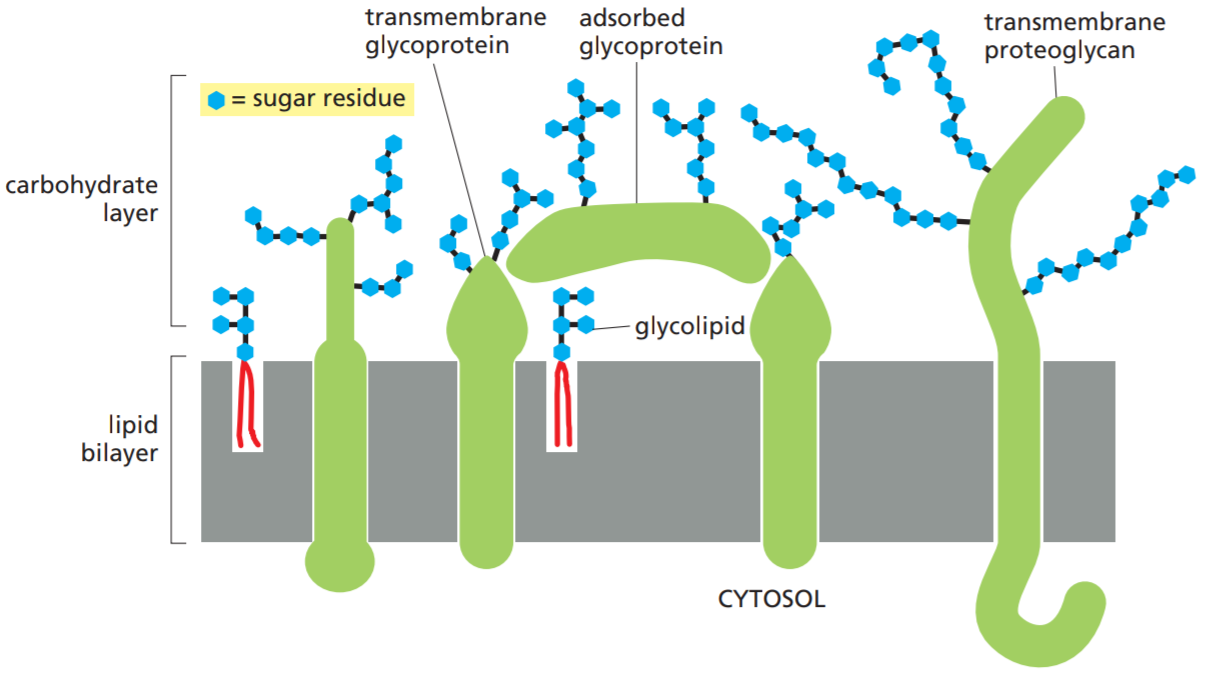
\includegraphics[scale=0.45]{images/figure_10_25.png}
        \end{center}
        \vspace{-20pt}
        \item The carbohydrate layer is made up of the oligosaccharide side chains of membrane glycolipids and membrane glycoproteins and the polysaccharide chains on membrane proteoglycans. In addition, adsorbed glycoproteins, and adsorbed proteoglycans (not shown), contribute to the carbohydrate layer in many cells.
        \item \textbf{Lectins}: carbohydrate-binding proteins that are highly specific for sugar groups of other molecules.\par 
        \item Lectins have a role in recognition on the cellular and molecular level and play numerous roles in biological recognition phenomena involving cells, carbohydrates, and proteins. 
    \end{itemize}

    \subsection*{Membrane Proteins Can Be Solubilized and Purified in Detergents}
    \begin{itemize}
        \item \textbf{Detergents}: are small amphiphilic molecules of variable structure that disrupt hydrophobic associations and destroy the lipid bilayer, which can solubilize membrane proteins.
        \item At low concentration, detergents are monomeric in solution, but when their concentration is increased above a threshold, called the critical micelle concentration (CMC), they aggregate to form micelles.
        \item When mixed with membranes, the hydrophobic ends of detergents bind to the
        hydrophobic regions of the membrane proteins, where they displace lipid molecules with a collar of detergent molecules.
    \end{itemize}

    \subsection*{Bacteriorhodopsin Is a Light-driven Proton H\bfg{^+} Pump That
    Traverses the Lipid Bilayer as Seven \bfg{\alpha} Helices}
    \begin{itemize}
        \item \textbf{Bacteriorhodopsin}: a protein used by Archaea, most notably by halobacteria, a class of the Euryarchaeota.
        \item Bacteriorhodopsin acts as a proton pump; that is, it captures light energy and uses it to move protons across the membrane out of the cell.
    \end{itemize}

    \subsection*{The Cortical Cytoskeleton Gives Membranes Mechanical Strength and Restricts Membrane Protein Diffusion}
    \begin{itemize}
        \item \textbf{Spectrin}: a long, thin, flexible rod about 100 nm in length and is a cytoskeletal protein that lines the intracellular side of the plasma membrane in eukaryotic cells.  
        \item \textbf{Cortex}: also known as the actin cortex or actomyosin cortex, is a specialized layer of cytoplasmic proteins on the inner face of the cell membrane.
        \item The protein constituents of the cortex undergo rapid turnover, making the cortex both mechanically rigid and highly plastic, two properties essential to its function.
    \end{itemize}

    \subsection*{Membrane-bending Proteins Deform Bilayers}
    \begin{itemize}
        \item In many cases, membrane shape is influenced by dynamic pushing and pulling forces exerted by cytoskeletal or extracellular structures.
        \item \textbf{Membrane bending proteins}: Proteins that control membrane curvature and play a crucial part in producing deformations needed to create cell structures.
        \item Currently there are 4 (the book lists 3) proposed mechanisms to explain protein-mediated membrane bending:
            \begin{itemize}[label=$\circ$]
                \item Lipid clustering: Bacterial toxins that favor binding, and thus clustering of certain lipid molecules, give rise to membrane curvature when factoring particular lipids involved.
                \item Protein forms rigid scaffold: proteins that deform the membrane or stabilize an already bent membrane.
                \item Insertion of amphipathic domains: Some insert hydrophobic protein domains or attached lipid anchors into one of the leaflets of a lipid bilayer. Increasing the area of only one leaflet causes the membrane to bend.
                \item Protein crowding (not in book): When a high enough local concentration of protein is present on membrane surface, repulsion between protein molecules on the membrane surface can induce membrane curvature. A recent study even shows that protein crowding can cause membrane bending and leads to membrane fission.
            \end{itemize}
        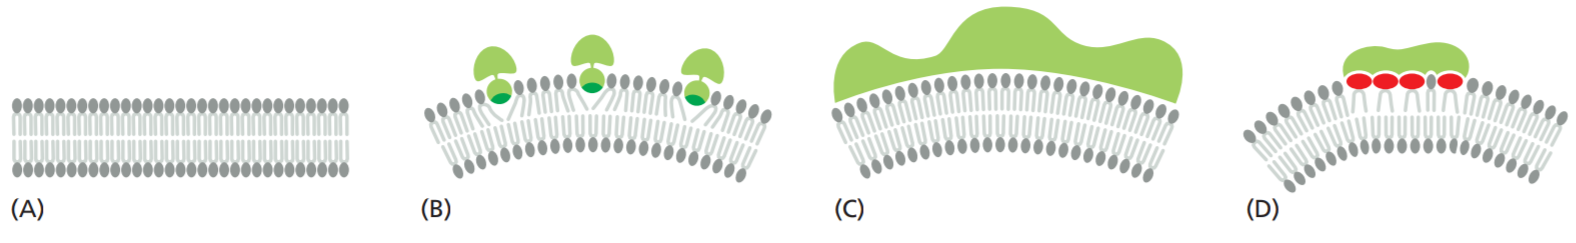
\includegraphics[width=\linewidth]{images/figure_10_40.png}
        \item (A) Bilayer without protein bound. 
        \item (B) A hydrophobic region of the protein can insert as a wedge into one monolayer to pry lipid head groups apart. Such regions can either be amphiphilic helices as shown or hydrophobic hairpins. 
        \item (C) The curved surface of the protein can bind to lipid head groups and deform the membrane or stabilize its curvature. 
        \item (D) A protein can bind to and cluster lipids that have large head groups and thereby bend the membrane. 
    \end{itemize}

    \begin{probbox}{Membrane Proteins: Summary}
        Whereas the lipid bilayer determines the basic structure of biological membranes, proteins are responsible for most membrane functions, serving as specific receptors, enzymes, transporters, and so on. Transmembrane proteins extend across the lipid bilayer. Some of these membrane proteins are single-pass proteins, in which the polypeptide chain crosses the bilayer as a single \(\alpha\)-helix. Others are multipass proteins, in which the polypeptide chain crosses the bilayer multiple times---either as a series of \(\alpha\)-helices or as a \(\beta\)-sheet rolled up into the shape of a barrel. All proteins responsible for the transport of ions and other small water-soluble molecules through the membrane are multipass proteins. Some membrane proteins do not span the bilayer but instead are attached to either side of the membrane: some are attached to the cytosolic side by an amphipathic a helix on the protein surface or by the covalent attachment of one or more lipid chains, others are attached to the noncytosolic side by a GPI anchor. Some membrane-associated proteins are bound by noncovalent interactions with transmembrane proteins. In the plasma membrane of all eukaryotic cells, most of the proteins exposed on the cell surface and some of the lipid molecules in the outer lipid monolayer have oligosaccharide chains covalently attached to them. Like the lipid molecules in the bilayer, many membrane proteins are able to diffuse rapidly in the plane of the membrane. However, cells have ways of immobilizing specific membrane proteins, as well as ways of confining both membrane protein and lipid molecules to particular domains in a continuous lipid bilayer. The dynamic association of membrane-bending proteins confers on membranes their characteristic three-dimensional shapes.
    \end{probbox}
}\end{secbox}
%\endgroup
%  ^^^^^^^^^^^^^^^^^^^^^^^^^^^^^^^^^   Section 10.2   ^^^^^^^^^^^^^^^^^^^^^^^^^^^^^^^^^  %  
%%%%%%%%%%%%%%%%%%%%%%%%%%%%%%%%%%%%%%%%%%%%%%%%%%%%%%%%%%%%%%%%%%%%%%%%%%%%%%%%%%%%%%%%%%
\end{document}